\documentclass[12pt,a4paper]{article}
\usepackage[]{listings}
%packages used
\usepackage[english]{babel}
\usepackage[margin=1in,  left=1.25in]{geometry} %margins
\usepackage{pslatex}%Times new roman font
\usepackage{graphicx}%for images
\usepackage{float}
%\usepackage{fancyhdr}
%\pagestyle{fancy}
%\fancyfoot{}

%beginning of document
\begin{document}
%declaration page
%\thispagestyle{empty}
\pagenumbering{roman} 
\begin{titlepage}
  \begin{center}
    \vspace*{1cm}

    \textbf{\Huge pipelined CPU  report}

    \vspace{0.5cm}

         
    \vspace{1.5cm}

    \textbf{\large Chang Zihao \\20206018\\\large Cui Yuxuan\\20206019}

    \vfill
         

         
    \vspace{0.8cm}
  


         
\end{center}
\end{titlepage}


\newpage
%table of contents
\tableofcontents
\thispagestyle{empty}

\newpage
\pagenumbering{arabic}
\setcounter{page}{1}

\section{Introduction}

Lab5 is required to design a pipelined CPU.
A pipelined CPU processes five stage.
And use pipelined to save time.
Then deal with the data hazard and control hazard.

\subsection{Data Path}

\begin{enumerate}
\item Update the PC to hold the address of the next instruction and fetch the instruction at the address in PC.
\item Decode the instruction.
\item Execute the instruction.
\item Save data into the memory.
\item Use bypass unit to solve the data hazard.
\item We use  “always-not-taken” branch predictor to solve the control hazard.
\end{enumerate}

\subsection{Control-pipelined}

\begin{enumerate}
\item Operation to be performed by ALU.
\item Whether register file needs to be written.
\item Signals for multiple intermediate multiplexors.
\item Whether data memory needs to be written. 
\item Control signal send on time at the first stage, then use register to send control signal to the module at the next stage. 
\end{enumerate}

\newpage

\section{Design}

As the Description of TB file mentioned, We do not need to implement memory and register ourselves.
So we design the path to connect them together.
Then we have to design some necessary modules.

\subsection{Module design}

\subsubsection{ALU module}

ALU has been designed in lab1.
But this time we need to modify the ALU slightly.
At the beginning, I took out the Cout alone to deal specifically with branch instructions
It works, but not necessary.
So I put the Cout back and cancel it.


\subsubsection{PC module}

The PC is a state element that holds the address of the current instruction. 
It is updated at the end of every clock cycle.

\subsubsection{add module}

The adder is responsible for incrementing the PC to hold the address of the next instruction.
It takes two input values, adds them together, and outputs the result

\subsubsection{Sign extend module}

Single extend module is used to increase the number of bits of a binary number while preserving the number's sign and value. 

\subsubsection{MUX module}

Mux, a data selector, which was used to select which the single will be output.

\newpage

\section{Implementation}

The whole circuit was shown below.

\begin{figure}[H]
  \centering
  \includegraphics[height=5in, angle=90]{datapath.JPG}
  \end{figure}
%There might be something different with the circuit.
%  \begin{figure}[H]
%    \centering
%    \includegraphics[height=3.5in]{cont.jpg}
%    \end{figure}
\newpage

\section{Evaluation}

I pass all the test in the testbench folder.

\begin{figure}[H]
  \centering
  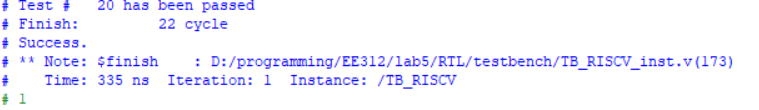
\includegraphics[height=1in]{inst.png}
  \end{figure}

\begin{figure}[H]
  \centering
  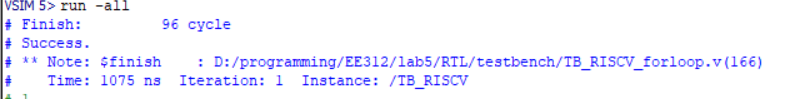
\includegraphics[height=1in]{forloop.png}
  \end{figure}

  \begin{figure}[H]
    \centering
    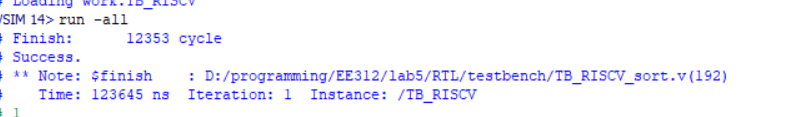
\includegraphics[height=1in]{sort.png}
    \end{figure}

% We first encountered some problems in understanding the meaning of the question, 
% but in the end by looking at the test code, 
% we thoroughly understood the meaning of the question.
% And at last, we pass all the test and finished the whole project.
% I hope that future projects will give enough time to think and complete the code.

\section{Conclusion}

The pipelined CPU is quicker than single-cycle CPU and multi-cycle CPU, but it is more difficult than single-cycle CPU and multi-cycle CPU.
\end{document}
